
\section*{Ejercicios}
\addcontentsline{toc}{section}{Ejercicios}

\begin{Ejercicio}{Cálculo de $\Sn$, $u_{em}$ y $\Jn \cdot \En$ en solenoide de intensidad variable.}
    Sea un solenoide de radio $a$ con $n$ vueltas por unidad de longitud y intensidad 
    \begin{equation}
        I = I_0 \frac{t}{\tau}
    \end{equation}
    Calcula $\Sn$ dentro y fuera del solenoide, y compáralo con $u_{em}$ y $\Jn \cdot \En$.
\end{Ejercicio}

Lo primero que tenemos que calcular es el campo magnético, a través de las ecuaciones de Maxwell:

\begin{equation}
    \Div \Bn = 0  \qquad \Curl \Bn  = - \mu_0 \Jn 
\end{equation}
(en realidad esta sería la componente $\Bn$ generada únicamente por la carga, también deberíamos tener en consideración el campo eléctrico). En este caso tendremos una corriente superficial en el sentido $\varphin$, tal que: 


\begin{equation}
    \Kn = n I(t) \varphin 
\end{equation}
Luego tenemos qeu aplicar el teorema de Stokes:

\begin{equation}
    \int_S \Curl \Bn  \cdot  \D \Sn= \oint_C \Bn \cdot  \D \lnn  \to 
    \int_S \Jn \cdot \D \Sn = \oint_C \Bn  \cdot \D \lnn
\end{equation}
Dado que $\Div \Bn = 0$, tenemos que $\Bn$ solo puede tener dos direcciones: $\varphin$ y $\hnz$. Si además tenemos que $\Curl \Bn = \mu_0 \Jn$ y $\Jn \propto \varphin$, tenemos que $\Bn \propto \hnz$. Debido al propio teorema de Stokes se cumple que $B\neq B(\rho,z,\varphi)$, es decir, debe ser una constante, tanto dentro como fuera del solenoide. Debido también a que $B=0$ en el infinito, tenemos que $\Bn = 0$ fuera del solenoide. Así pues, en el interior del solenoide tenemos un campo uniforme en la dirección $\hnz$: $\Bn = B_0 \hnz$. Tenemos pues que:

\begin{equation}
    B_0 = \mu_0 n I(t) \to \Bn = \mu_0 n I(t) \hnz 
\end{equation}
Ahora el campo eléctrico: 

\begin{equation}
    \Curl \En = - \pdv{\Bn}{t}
\end{equation}
y como $\Div \En = 0$, tenemos pues que $\En \propto \hnz$. Por simetría azimutal y en el eje z, solo puede depender de la dirección radial $r$, i.e. $\En = E(r) \hnz$. Así pues, el campo eléctrico depende de si estamos en el interior o exterior

\begin{equation}
    E(r) 2\pi \rho =  \dot{\Bn} \qquad \text{si} \ r<a
\end{equation}
Dado que $\Div \Bn = 0$, tenemos que $\Bn$ solo puede tener dos direcciones: $\varphin$ y $\hnz$. Si además tenemos que $\Curl \Bn = \mu_0 \Jn$ y $\Jn \propto \varphin$, tenemos que $\Bn \propto \hnz$. Debido al propio teorema de Stokes se cumple que $B\neq B(\rho,z,\varphi)$, es decir, debe ser una constante, tanto dentro como fuera del solenoide. Debido también a que $B=0$ en el infinito, tenemos que $\Bn = 0$ fuera del solenoide. Así pues, en el interior del solenoide tenemos un campo uniforme en la dirección $\hnz$: $\Bn = B_0 \hnz$. Tenemos pues que:

\begin{equation}
    B_0 = \mu_0 n I(t) \to \Bn = \mu_0 n I(t) \hnz 
\end{equation}
Ahora el campo eléctrico: 

\begin{equation}
    \Curl \En = - \pdv{\Bn}{t}
\end{equation}
y como $\Div \En = 0$, tenemos pues que $\En \propto \varphin$. Por simetría azimutal y en el eje z, solo puede depender de la dirección radial $r$, i.e. $\En = E(r) \varphin$. Así pues, el campo eléctrico depende de si estamos en el interior o exterior

\begin{align}
    \En(r) =  - \frac{r}{2}  \mu_0 n \dot{I} \varphin \quad \Bn = \mu_0 n I(t) \hnz  & \qquad \text{si} \ r<a \\
    \En(r) =  - \frac{a^2}{2r}  \mu_0 n \dot{I} \varphin \quad  \Bn = 0 & \qquad \text{si} \ r>a
\end{align}
Estudianmos $\Sn$ en función del punto. Veamos que:

\begin{align}
    \Sn = - \frac{r}{2} I(t) \dot{I} \rhon & \quad \text{si}  \ r<a \\
    \Sn = 0  & \quad \text{si}  \ r>a
\end{align}
Por otro lado: 


\begin{align}
    u_{em} = \frac{\epsilon_0}{2} \bqty{\frac{r}{2} \mu_0  \dot{I} }^2 + \frac{1}{2 \mu_0} \bqty{\mu_0  {I}}^2 & \quad \text{si}  \ r<a  \\
    u_{em} = \frac{\epsilon_0}{2} \bqty{\frac{r}{2} \mu_0  \dot{I} }^2  & \quad \text{si}  \ r>a
\end{align}
De lo que se deduce que fuera $\pdv{u_{em}}{t}=0$. Así pues, solo existe un flujo de energía $\Sn$ dentro del solenoide, que se pierde en el efecto joule y en la densidad de energía $u_{em}$. Veamos que

\begin{equation}
    \Jn \cdot \En =  \frac{a}{2} \mu_0  I \dot{I}
\end{equation}

%
%
%
%
%
%
%
%
%
%
%
%
%
%
%
%
%
%
%
%
%
%
%
%
%


\begin{Ejercicio}{Cálculo de $\Fn$ en el caso de ondas incidentes en un medio dieléctrico.}
    Sea una onda incidente con campos $\En,\Bn$ tal que
    \begin{equation}
        \En_i = E_i \hnx e^{i(kz-wt)} \qquad 
        \Bn_i = \frac{E_i}{c} \hny e^{i(kz-wt)}
    \end{equation}
    Cálculese la fuerza y el vector de Poyting en todos los puntos.
\end{Ejercicio}

Tenemos que considerar las condiciones de frontera para hallar los campos reflejados y trasmitidos, pues:

\begin{center}
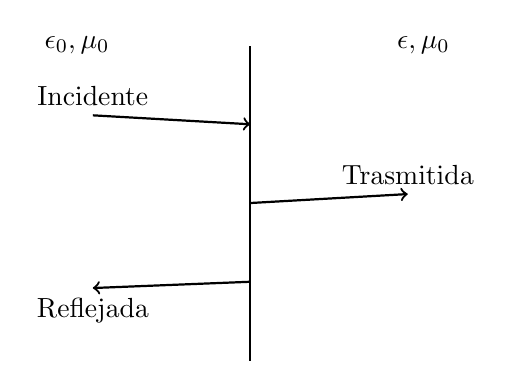
\begin{tikzpicture}[scale=2]
    \node (Ei) at (-1,0.68) {Incidente};
    \node (Er) at (-1,-0.68) {Reflejada};
    \node (Et) at (1,0.18) {Trasmitida};


    \node (epsilon0) at (-1.1,1) {$\epsilon_0,\mu_0$};
    \node (epsilon) at (1.1,1) {$\epsilon, \mu_0$};
    %\node[opciones] (nombre) at (x,y) {contenido};

    \draw[thick] (0,-1) -- (0,1);
    \draw[arrows={->},thick] (Ei.south) -- (0,0.5);
    \draw[arrows={<-},thick] (Er.north) -- (0,-0.5);
    \draw[arrows={<-},thick] (Et.south) -- (0,0);
\end{tikzpicture}
\end{center}
Los campos entonces

\begin{equation}
    \En_i = E_i \hnx e^{i(kz-wt)} \qquad 
    \Bn_i = \frac{E_i}{c} \hny e^{i(kz-wt)}
\end{equation}
\begin{equation}
    \En_r = E_r \hnx e^{i(-kz-wt)} \qquad 
    \Bn_r = -\frac{E_r}{c} \hny e^{i(-kz-wt)}
\end{equation}
\begin{equation}
    \En_t = E_t \hnx e^{i(kz-wt)} \qquad 
    \Bn_t = \frac{E_t}{v} \hny e^{i(kz-wt)}
\end{equation}
las condiciones de frotnera son:
\begin{equation}
    \hnn \times (\En_2 - \En_1) = 0
\end{equation}
\begin{equation}
    \hnn \times ( \Bn_2 - \Bn_1) = 0
\end{equation}
Lo que nos lleva a las siguientes ecuaciones acopladas que relacionan $E_i,E_t$ y $E_r$:

\begin{equation}
    \left\lbrace
    \begin{array}{rl}
        E_i + E_r - E_t & = 0 \\[1.3em]
        {\sqrt{\epsilon_0}}{E_i} -{\sqrt{\epsilon_0}}{E_r}  -{\sqrt{\epsilon}}{E_t} & = 0 
    \end{array}  
    \right\rbrace \Rightarrow
    {2\sqrt{\epsilon_0}}{E_i} = E_t \bqty{{\epsilon_0} + {\epsilon}} 
    \Rightarrow 
     E_t = \frac{2\sqrt{\epsilon_0}}{\sqrt{\epsilon_0} + \sqrt{\epsilon}} E_i 
\end{equation}
y la parte reflejada es: 


\begin{equation}
    E_r = -\frac{\sqrt{\epsilon} -\sqrt{\epsilon_0}}{\sqrt{\epsilon}+\sqrt{\epsilon_0}}E_i
\end{equation}
Usamos $\beta = \sqrt{\varepsilon/\varepsilon_0}$:

\begin{equation}
    E_t = \frac{2}{1 + \beta} E_i  \qquad 
    E_r = \frac{1 - \beta}{1 + \beta}E_i
\end{equation}
que lógicamente podemos multiplicar y dividir por $\sqrt{\mu_0}$ y por tanto poder expresarlo en términos de la velocidad de la luz en el medio o incluso el índice de refracción. Lógicamente para calcular la fuerza que se ejerce tendremos que considerar un volumen, tal que: 

\begin{center}
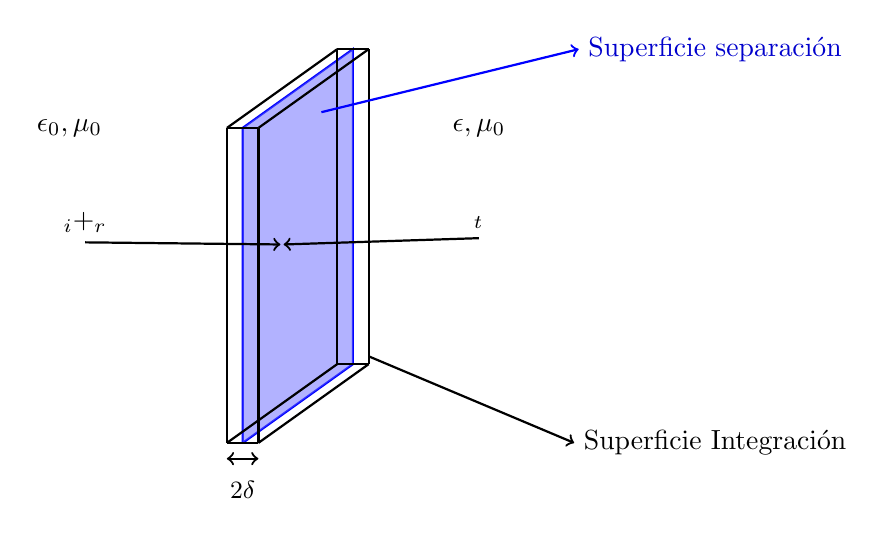
\begin{tikzpicture}[scale=2]
    \node (Ei) at (-1,0.4) {$\Fn_i+\Fn_r$};
    %\node (Er) at (-1,-0.68) {$\Fn_t$};
    \node (Et) at (1.5,0.4) {$\Fn_t$};


    \node (epsilon0) at (-1.1,1) {$\epsilon_0,\mu_0$};
    \node (epsilon) at (1.5,1) {$\epsilon, \mu_0$};
    %\node[opciones] (nombre) at (x,y) {contenido};

    % Superficie de separacion

    \draw[thick,blue] (0.0,-1) -- (-0.0,1) -- (0.7,1.5) -- (0.7,-0.5) -- (0.0,-1);
    \fill[blue!60, opacity=0.5] (0.0,-1) -- (-0.0,1) -- (0.7,1.5) -- (0.7,-0.5) -- (0.0,-1);


    % Ondas incidentes/reflejadas7/trasmitidas:

    \draw[arrows={->},thick] (Ei.south) -- (0.24,0.26);
    %\draw[arrows={->},thick] (Er.north) -- (-0.2,-0.5);
    \draw[arrows={->},thick] (Et.south) -- (0.26,0.26);


    % Superficies: 

    \draw[thick] (0.1,-1) -- (0.1,1);
    \draw[thick] (-0.1,-1) -- (-0.1,1);
    \draw[thick] (-0.1,-1) -- (0.1,-1);
    \draw[thick] (-0.1,1) -- (0.1,1);

    
    \draw[thick] (-0.1,1) -- (0.6,1.5);
    \draw[thick] (0.1,1) -- (0.8,1.5);
    \draw[thick] (0.6,1.5) -- (0.8,1.5);
    \draw[thick] (0.6,1.5) -- (0.8,1.5);

    \draw[thick] (-0.1,-1) -- (0.6,-0.5);
    \draw[thick] (0.1,-1) -- (0.8,-0.5);
    \draw[thick] (0.6,-0.5) -- (0.8,-0.5);


    \draw[thick] (0.8,-0.5) -- (0.8,1.5);
    \draw[thick] (0.6,-0.5) -- (0.6,1.5);

    % Distinción superficie/superficie de integración:

    \node[color=blue!80!black] (sep) at (3,1.5) {Superficie separación};
    \draw[thick,color=blue,arrows={->}] (0.5,1.1) -- (sep.west);

    \node[color=black!80!black] (sep2) at (3,-1) {Superficie Integración};
    \draw[thick,color=black,arrows={->}] (0.8,-0.45) -- (sep2.west);


    \draw[thick,arrows={<->}] (-0.1,-1.1) -- (0.1,-1.1);
    \node (selta) at (0.0,-1.3) {\small $2\delta$};


\end{tikzpicture}
\end{center}

Tenemos que integrar en la superficie de arriba, cuyo $2\delta \to 0$. Así pues, la fuerza la calculamos como:

\begin{equation}
    \Fn = \oint \langle \Tt \rangle \D \Sn 
\end{equation}
y dado que $\En,\Bn \perp \hnz$, tenemos que la fuerza puede describirse a través de
\begin{equation}
    \Fn =  \int \langle \Tt_{i+r} \rangle (-\hnz) \D S + \int \langle \Tt_{t} \rangle (\hnz) \D S
\end{equation}
donde el tensor, con un abuso de notación, es ahora mismo este escalar: 
\begin{equation}
    \Tt = \epsilon \frac{|E|^2}{2} + \frac{1}{\mu_0} \frac{|B|^2}{2}
\end{equation}
Esto nos lleva básicamente a: 
\begin{equation}
    \Fn = \hnz  \int \pqty{ \langle \Tt_{i+r} \rangle - \langle \Tt_{t} \rangle  } \D S 
\end{equation}
y dado que los tensores/campos no dependen de $x,y$, podemos sacarlos a fuera, y toda la fuerza dependerá de: 
\begin{equation}
    \Fn = \hnz  \int \pqty{ \langle \Tt_{i+r} \rangle - \langle \Tt_{t} \rangle} \D S 
\end{equation}
Si ahora desarrollamos los tensores (que ya hemos indicado que eran escalares), teniendo en cuenta que son \textit{promedios temporales}
\begin{equation}
    \left\langle\frac{\Fn}{S} \right\rangle = \hnz \pqty{\epsilon_0 \left\langle \frac{|E_{i+r}|^2}{2} \right\rangle + \frac{1}{\mu_0} \left\langle \frac{|B_{i+r}|^2}{2}  \right\rangle - 
    \epsilon  \left\langle \frac{|E_{t}|^2}{2} \right\rangle - \frac{1}{\mu_0} \left\langle \frac{|B_{t}|^2}{2} \right\rangle}  
\end{equation}
En este caso hay que tener en cuenta \textit{la diferencia de signos en las exponenciales de los campos reflejados}. Así pues ($\sqrt{\varepsilon/\varepsilon_0}$): 

\begin{equation}
   \left\langle |E_{i+r}|^2 \right\rangle = \bqty{1 + \pqty{\frac{1-\beta}{1+\beta}}^2 + 2\pqty{\frac{1-\beta}{1+\beta}} \cos (2kz)} |E_i|^2 = \bqty{\pqty{\frac{2 + 2\beta^2}{(1+\beta)^2}} + 2\pqty{\frac{1-\beta}{1+\beta}} \cos (2kz)} |E_i|^2
\end{equation}
\begin{equation}
   \left\langle |B_{i+r}|^2 \right\rangle = \sqrt{\epsilon_0 \mu_0}  \bqty{\pqty{\frac{2 + 2\beta^2}{(1+\beta)^2}} - 2\pqty{\frac{1-\beta}{1+\beta}} \cos (2kz)} |E_i|^2
\end{equation}
\begin{equation}
   \left\langle |E_{t}|^2 \right\rangle =\pqty{\frac{2}{1+\beta}}^2  |E_i|^2  \qquad
   \left\langle |B_{t}|^2 \right\rangle = \sqrt{\epsilon_0 \mu_0 } \pqty{\frac{2}{1+\beta}}^2 |E_i|^2
\end{equation}
Así pues: 

\begin{equation}
    \left\langle \frac{\Fn}{S} \right\rangle = \hnz \bqty{\frac{\beta^2 - 2 \beta + 1}{(1+\beta)^2}} 2\epsilon_0 |E_i|^2 =  \hnz\bqty{\frac{(1-\beta)^2}{(1+\beta)^2}} 2\epsilon_0 |E_i|^2 
\end{equation}
